\documentclass[tikz,border=10pt]{standalone}
\begin{document}
  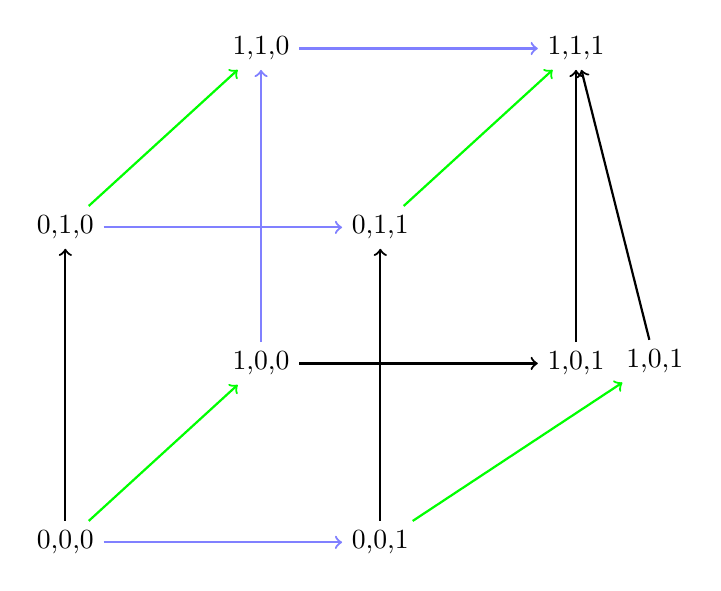
\begin{tikzpicture}[node distance=4cm, align=center]
    \title{unfolded HDA}
    % face 1
    \node(q00)                  {0,0,0};
    \node(q01) [right of=q00]   {0,0,1};

    \node(q02) [above of=q00]   {0,1,0};

    \node(q03) [above of=q01]   {0,1,1};
    
    % face 2
    \node(q04) [above right=2cm] {1,0,0};
    \node(q05) [right of=q04] {1,0,1};

    \node(q06) [above of=q04] {1,1,0};
    \node(q07) [above of=q05] {1,1,1};

    %extra
    \node(q05x) [above=2.3cm, right=7cm] {1,0,1};



    %%%%% Edges Figure 1 %%%%%
    %face 1(1D)
    \draw[->][draw=blue!50, thick](q00) to node [below] {} (q01);
    \draw[->][draw=black, thick](q00) to node [below] {} (q02);
    \draw[->][draw=green, thick](q00) to node [below] {} (q04);

    \draw[->][draw=black, thick](q01) to node [below] {} (q03);
    \draw[->][draw=green, thick](q01) to node [below] {} (q05x);

    \draw[->][draw=blue!50, thick](q02) to node [below] {} (q03);
    \draw[->][draw=green, thick](q02) to node [below] {} (q06);

    \draw[->][draw=black, thick](q04) to node [below] {} (q05);
    \draw[->][draw=blue!50, thick](q04) to node [below] {} (q06);

    \draw[->][draw=green, thick](q03) to node [below] {} (q07);

    \draw[->][draw=black, thick](q05) to node [below] {} (q07);
    \draw[->][draw=black, thick](q05x) to node [below] {} (q07);

    \draw[->][draw=blue!50, thick](q06) to node [below] {} (q07);

  \end{tikzpicture}
\end{document}